%! TeX program = lualatex
\documentclass[../main.tex]{subfiles}
\begin{document} 
\section{Vectors}

We have been looking at models involving one quantity, e.g., the population of a group of unicorns.  We now develop mathematical tools (\emph{linear} vector fields and \emph{linear} systems of differential equations) to model systems involving two or more quantities, e.g., an ecosystem involving a predator and prey.

We use an introductory example to demonstrate why vectors are useful in science.
\begin{example}
  Consider an ecosystem involving orcas (predators) and seals (preys). Their population over time (in years) is presented as a table. 

  \begin{table}[H]
    \centering
    \begin{tabular}{r|c|c|c|c}
      time  & \(0\) & \(1\) & \(2\) & \(3\)  \\\midrule
      orcas & \(5\) & \(6\) & \(4\) & \(3\)  \\
      seals & \(5\) & \(3\) & \(2\) & \(4\)  \\
    \end{tabular}
  \end{table}

  \begin{center}
    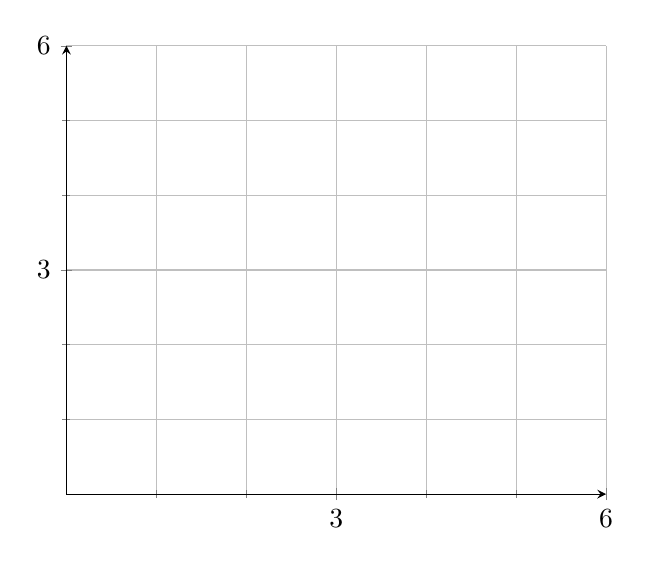
\begin{tikzpicture}[scale=1]
      \begin{axis}[xmin=0, xmax=6, ymin=0, ymax=6, enlargelimits, grid=both, minor tick num=2, axis lines=middle, xtick={0, 3, 6}, ytick={0, 3, 6}]
      \end{axis}
    \end{tikzpicture}
    \quad
    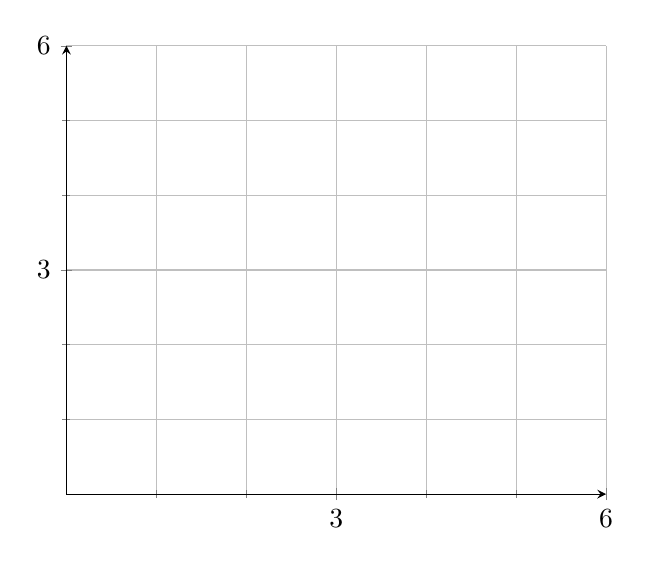
\begin{tikzpicture}[scale=1]
      \begin{axis}[xmin=0, xmax=6, ymin=0, ymax=6, enlargelimits, grid=both, minor tick num=2, axis lines=middle, xtick={0, 3, 6}, ytick={0, 3, 6}]
      \end{axis}
    \end{tikzpicture}
  \end{center}
\end{example}

\blanklines{8}

\begin{definition}[vectors]
  A (state) \hlmain{vector} \(\vec{x}\) is an ordered list of numbers
  \[
    \vec{x} = 
    \begin{bmatrix}
      x_{1} \\ x_{2} \\ \vdots \\ x_{n}
    \end{bmatrix}
    = 
    \begin{bmatrix}
      x_{1} & x_{2} & \cdots & x_{n}
    \end{bmatrix}^{T}.
  \]

  The number of rows in \(\vec{x}\) (zeros included) is called the \hlmain{dimension} (or the \hlmain{length}) of \(\vec{x}\).  Two vectors \(\vec{u}, \vec{v}\) are \hlmain{equal} if they have the same dimension and \(u_{1} = v_{1}, \ldots., u_{n} = v_{n}\).
\end{definition}
Depending on the application, a vector can be visualized as a point or as an arrow as shown above.

\clearpage

\section{Algebraic operations on vectors}

We now study vectors abstractly and quickly introduce all fundamental operations on vectors. \medskip

\begin{itemize}[wide]

  \item Every vector has a \hlmain{direction} and a \hlmain{length}. The direction is implicit, but the length \(\|\vec{v}\|\) is defined by the Pythagorean theorem:
    \begin{equation}
      \| \vec{v} \| = \sqrt{ (v_{1})^{2} + \cdots + (v_{n})^{2} }.
    \end{equation}
    \blanklines{5}

  \item We can multiply a \hlsupp{constant \(c\)} by a \hlmain{vector \(\vec{v}\)}, and \hlmain{add two vectors} having the same dimension.
    \begin{equation}
      \hlsupp{c}\, \hlmain{\vec{v}}
      = 
      \hlsupp{c}
      \begin{bmatrix}
        \hlmain{v_{1}} \\ \hlmain{v_{2}} \\ \vdots \\ \hlmain{v_{n}}
      \end{bmatrix}
      =
      \begin{bmatrix}
        \hlsupp{c}\, \hlmain{v_{1}} \\ \hlsupp{c}\, \hlmain{v_{2}} \\ \vdots \\ \hlsupp{c}\, \hlmain{v_{n}}
      \end{bmatrix}
      \quad\text{and}\quad
      \hlmain{\vec{u} + \vec{v}}
      =
      \begin{bmatrix}
        u_{1} \\ u_{2} \\ \vdots \\ u_{n}
      \end{bmatrix}
      +
      \begin{bmatrix}
        v_{1} \\ v_{2} \\ \vdots \\ v_{n}
      \end{bmatrix}
      =
      \begin{bmatrix}
        u_{1} + v_{1} \\ v_{2} + v_{2} \\ \vdots \\ u_{n} + v_{n}
      \end{bmatrix}.
    \end{equation}

    \blanklines{5}

    \includegraphics{../standalones/build/plot-RR2}
    \quad
    \includegraphics{../standalones/build/plot-RR2}
    \quad
    \includegraphics{../standalones/build/plot-RR2}

    \faStar{} In the operation \(c \, \vec{v}\), the constant \(c\) is called a \hlmain{scalar} because it stretches (aka scales) a vector's length without rotation.  The length of the stretched vector \(c \, \vec{v}\) is \underline{\hspace{2in}\phantom{\huge X}}.

  % \item The \hlmain{dot product} \(\vec{u} \bullet \vec{v}\) takes two vectors of the same dimension as input and outputs a scaler. 
  %   \begin{equation}
  %     \vec{u} \bullet \vec{v} = u_{1} v_{1} + \cdots + u_{n} v_{n}.
  %   \end{equation}
  %
  %   \blanklines{5}
\end{itemize}
\clearpage

A \hlmain{matrix} is an \(m\)-by-\(n\) array of numbers where \(m\) is the number of rows and \(n\) is the number of columns.  Moreover, if \(A\) is a matrix, then we write \(A_{ij}\) to represent the number in the \(i\)-th row and \(j\)-th column of the matrix \(A\). 
\blanklines{5}

In general, we can multiply an \(m\)-by-\(n\) matrix \(A\) by a \(n\)-dimensional vector \(\vec{v}\) to produce an \(n\)-dimensional vector \(\vec{u} = A\vec{v}\) whose entries are defined by
\[
  u_{i} = A_{i1} v_{1} + \cdots + A_{in} v_{n} 
  \quad\text{for each row index \(i = 1, \ldots, n\)}.
\]
\blanklines{5}

% The number of columns in \(A\) \hlwarn{must match} the number of rows in \(\vec{v}\).  Matrix-vector multiplication is defined by 
\faStar{} A main reason we study matricies is that matrix-vector multiplication can be used to encode system of linear equations in variable \(x_{1}, \ldots, x_{n}\) in the form \(A \vec{x} = \vec{b}\). 

We demonstrate this process through an example.

\begin{example}
  Write the following equations in the form \(A \vec{x} = \vec{b}\).
  \[
    \begin{array}{rcrcr}
      x_{1} &+& 0.2 x_{2} &=& 0.3 \\
      0.5 x_{1} &-& 0.3 x_{2} &=& 0.2
    \end{array}
  \]
  \blanklines{8}
\end{example}

\begin{example}
  Write the following matrix-vector equation as a system of linear equations.

  \[
    \begin{bmatrix}
      -1 & 3 \\
       2 & -1 
    \end{bmatrix}
    \begin{bmatrix}
      x_{1} \\
      x_{2}
    \end{bmatrix}
    =
    \begin{bmatrix}
      -1 \\
      3
    \end{bmatrix}
  \]
  \blanklines{8}
\end{example}
\clearpage

We can even encode recurrence using matrix-vector multiplication. 
\begin{example}
  Write the following system of recurrence equations in the form \(\vec{x}(t+1) = A \vec{x}(t)\).
  \[
    \begin{array}{rcrcr}
      x_{1}(t+1) &=& & & 0.5 x_{2}(t) \\
      x_{2}(t+1) &=& 0.2 x_{1}(t) &+& 0.3 x_{2}(t)
    \end{array}
  \]
  \blanklines{10}
\end{example}

\begin{example}
  Write \(\vec{x}(t+1) = A \vec{x}(t)\) as a system of recurrence equations where \(A = \begin{bmatrix} 0.2 & 0.8 \\ 0 & -0.7 \end{bmatrix}\).

  \blanklines{8}
\end{example}

An \hlmain{identity matrix} is a square matrix with \(1\)'s down the diagonal and \(0\) everywhere else, typically denoted as \(I_{n}\). The following are all identity matrices.
\[
  I_{2} = 
  \begin{bmatrix}
    1 & {\color{gray!30} 0} \\ 
    {\color{gray!30} 0} & 1
  \end{bmatrix},\quad
  I_{3} = 
  \begin{bmatrix}
    1 & {\color{gray!30} 0} & {\color{gray!30} 0} \\
    {\color{gray!30} 0} & 1 & {\color{gray!30} 0} \\
    {\color{gray!30} 0} & {\color{gray!30} 0} & 1
  \end{bmatrix},\quad
  I_{4} = 
  \begin{bmatrix}
    1 & {\color{gray!30} 0} & {\color{gray!30} 0} & {\color{gray!30} 0} \\
    {\color{gray!30} 0} & 1 & {\color{gray!30} 0} & {\color{gray!30} 0} \\
    {\color{gray!30} 0} & {\color{gray!30} 0} & 1 & {\color{gray!30} 0} \\
    {\color{gray!30} 0} & {\color{gray!30} 0} & {\color{gray!30} 0} & 1 \\
  \end{bmatrix}.
\]

Identity matricies are special because \hlmain{\(I_{n} A = A\) and \(I_{n} A = A\)} as long as \(A\) is an \(n \times n\) matrix. Moreover, \(I_{n} \vec{v} = \vec{v}\) as long as \(\vec{v}\) has \(n\) columns. In other words, \hlsupp{multiplication} by an identity matrix does nothing.  
\blanklines{5}
\end{document}
